\documentclass[12pt]{article}
\usepackage{amsmath}
\usepackage{geometry}
\usepackage{graphicx}
\usepackage[hidelinks]{hyperref}
\usepackage[latin1]{inputenc}
\usepackage{listings}
\usepackage[dvipsnames]{xcolor}
\renewcommand{\labelitemi}{$\textendash$}
\geometry{
    a4paper,
    total={170mm,257mm},
    left=20mm,
    right=20mm,
    top=15mm,
    bottom=15mm
}

\title{CS7DS2: Week 8 Assignment}
\author{Conor McCauley - 17323203}
\date{April 4, 2022}

\begin{document}

\maketitle

\section*{Functions}

The two functions that will be used during this assignment are:

$$f_1(x_0, x_1) = 9 (x_0 - 5)^4 + 10 (x_1 - 2)^2$$
$$f_2(x_0, x_1) = \max(x_0 - 5, 0) + 10 \cdot |x_1 - 2|$$

Their partial derivatives, as calculated in the week 2 assignment, are:

$$\frac{\partial f_1}{\partial x_0} = 36 (x_0 - 5)^3,\, \frac{\partial f_1}{\partial x_1} = 20x_1 - 40$$
$$\frac{\partial f_2}{\partial x_0} = \theta(x_0 - 5),\, \frac{\partial f_2}{\partial x_1} = 10\cdot sign(x_1 - 2)$$

\section*{Question (a)}

\noindent \textbf{(i)} The following snippet of code implements the global random search (GRS) algorithm. It begins by initialising the best function value found thus far to a large value. It then, for $N$ iterations, generates a random parameter vector $x$ with values of $x_i$ in the range $[l_i, u_i]$. At each iteration it tracks the best function value found and its associated parameter vector.

\lstset{basicstyle=\footnotesize}
\begin{lstlisting}[language=Python]
best_x = None
best_f = 1e20
for _ in range(N):
    this_x = [uniform(l[i], u[i]) for i in range(n)]
    this_f = f(*this_x)
    if this_f < best_f:
        best_x = deepcopy(this_x)
        best_f = this_f
\end{lstlisting}

\noindent \textbf{(ii)} For comparison, the gradient descent (GD) algorithm implemented in the week 2 assignment was used with $\alpha=0.01$. Running the GRS algorithm for $N$ iterations results in $N$ main function calls while running the GRS algorithm for $N$ iterations requires $N$ main function calls and $2N$ derivative function calls. The \texttt{timeit} module was used to test the average running times of both algorithms when $N = 200$. These running times were divided by the number of main function calls made to find their average times per evaluation. In order to fairly compare their results both the value of the function after each evaluation and the value of the function after each unit of time were plotted. The results for $f_1$ and $f_2$ can be seen in figures \ref{fig:a_ii_1} and \ref{fig:a_ii_2}, respectively.

\begin{figure}[h]
    \centering
    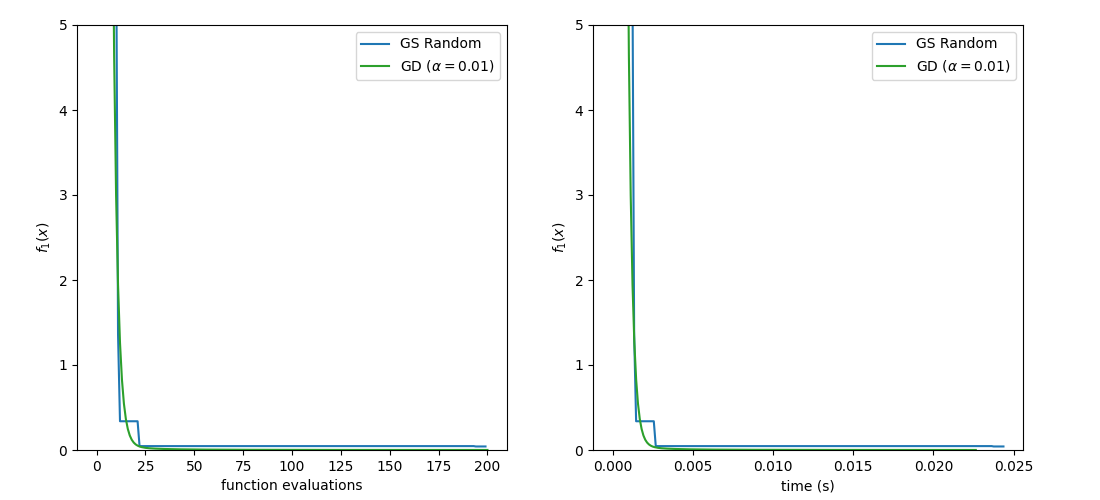
\includegraphics[scale=0.55]{figs/ab/a_ii_1.png}
    \caption{Change in $f_1(x)$ over evaluations and time (GD and GRS)}
    \label{fig:a_ii_1}
\end{figure}

For $f_1$, the GD algorithm manages to converge on the minimum in fewer than 50 iterations while the GSR algorithm, despite finding a fairly small value, fails to reach the same minimum. This is due to the low probability of choosing appropriate values for $x$ by random chance. Both algorithms required a similar amount of time to run so the second plot is irrelevant for this example.

\begin{figure}[h]
    \centering
    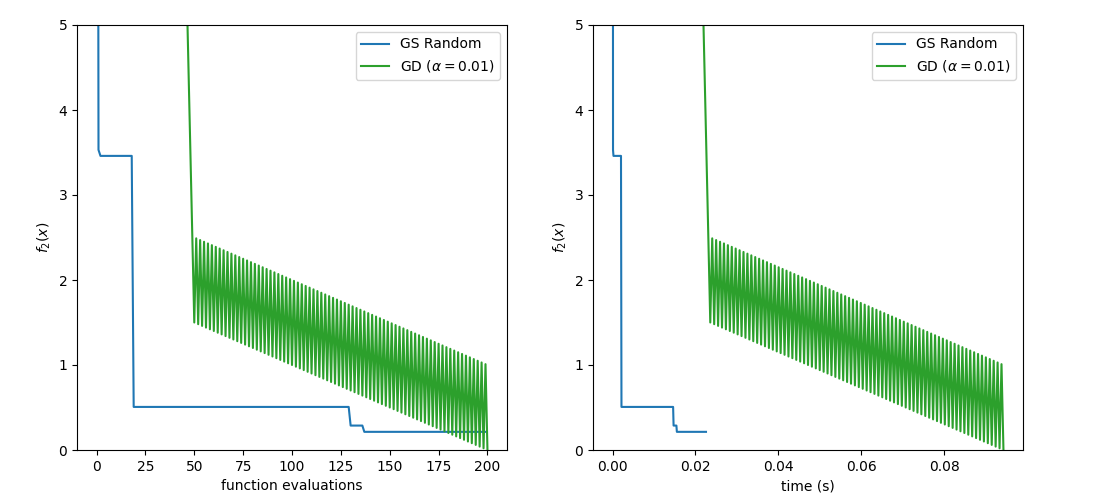
\includegraphics[scale=0.55]{figs/ab/a_ii_2.png}
    \caption{Change in $f_2(x)$ over evaluations and time (GD and GRS)}
    \label{fig:a_ii_2}
\end{figure}

For $f_2$, the GD algorithm fails to converge and instead oscillates back and forth toward the minimum due to $\alpha$ being too large. The GSR algorithm performs fairly well and reaches a small value without being entirely beaten by the GD algorithm. From the second plot it is clear that the GSR algorithm runs much faster for this function than the GD algorithm does. This is most likely due to the derivative function calls (made by the GD algorithm) requiring subsequent calls to two NumPy functions, \texttt{heaviside()} and \texttt{sign()}.

\section*{Question (b)}

\noindent \textbf{(i)} The following snippet of code implements the global population search (GPS) algorithm. It begins by generating a list of $N$ random parameter vectors $x$ and their corresponding function values. This process is similar to the one carried out in the GRS algorithm.

\lstset{basicstyle=\footnotesize}
\begin{lstlisting}[language=Python]
this_xs = [
    [uniform(l[i], u[i]) for i in range(n)]
    for _ in range(N)
]
this_fs = [f(*x) for x in this_xs]
\end{lstlisting}

Then, for a certain number of iterations it repeats the following process: select the best $M$ results from the list of $N$ vectors, for each of these $M$ best results, $m$, replace $\frac{N-M}{M}$ of the bottom $N - M$ results with a randomly perturbed version of $m$. The perturbation process involves multiplying each parameter in $m$ by a random value in the range $(0.8, 1.2)$.

\lstset{basicstyle=\footnotesize}
\begin{lstlisting}[language=Python]
num_new = (N - M) // M
for _ in range(num_iters):
    this_fs, this_xs = sort_lists(this_fs, this_xs)
    for i in range(M):
        this_x = this_xs[i]
        for j in range(num_new):
            pert_x = [x * uniform(0.8, 1.2) for x in this_x]
            k = M + (i * num_new) + j
            this_xs[k] = deepcopy(pert_x)
            this_fs[k] = f(*pert_x)
this_fs, this_xs = sort_lists(this_fs, this_xs)
\end{lstlisting}

\noindent \textbf{(ii)} For fairness, as in (a), the \texttt{timeit} library was used to test the average running time of the GPS algorithm when $N = 20, M = 5, num\_iters = 10$ which amounts to $N + num\_iters \cdot (N - M)$ function evaluations. The value of the function after each evaluation and the value of the function after each unit of time were plotted for the GPS, GRS and GD algorithms. These values for $f_1$ and $f_2$ can be seen in figures \ref{fig:b_ii_1} and \ref{fig:b_ii_2}, respectively. The change in $x$ for each algorithm was also plotted for each function and can been seen in figures \ref{fig:b_ii_1_cont} and \ref{fig:b_ii_2_cont}.

\begin{figure}[h]
    \centering
    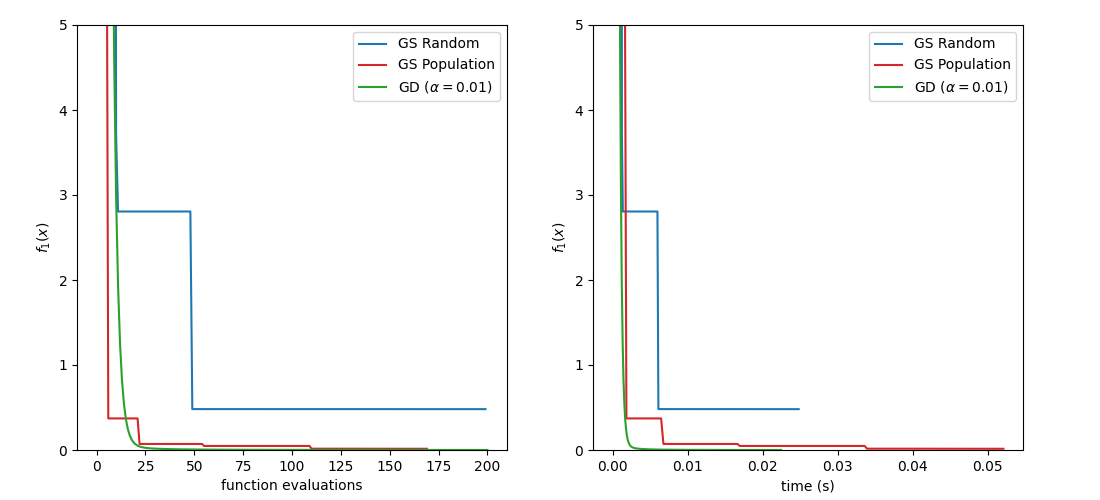
\includegraphics[scale=0.55]{figs/ab/b_ii_1.png}
    \caption{Change in $f_1(x)$ over evaluations and time (GD, GRS and GPS)}
    \label{fig:b_ii_1}
\end{figure}

For $f_1$, the GPS algorithm produces much better results than GRS with GD only slightly beating it. However, the GPS algorithm takes almost twice as long as the other two to run per evaluation.

\begin{figure}[h]
    \centering
    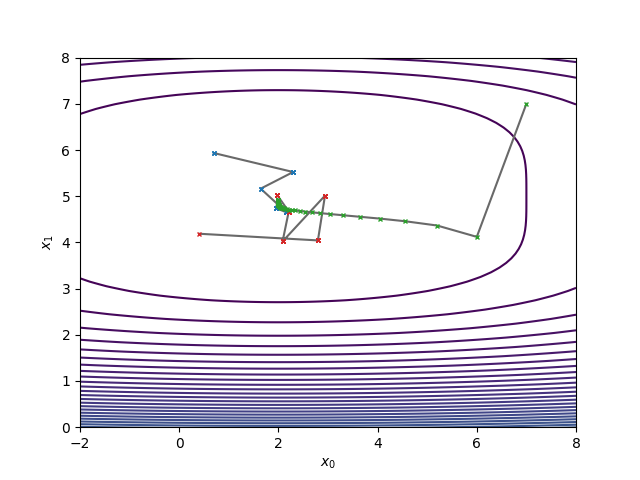
\includegraphics[scale=0.55]{figs/ab/b_ii_1_cont.png}
    \caption{Change in $x$ over evaluations (GD, GRS and GPS)}
    \label{fig:b_ii_1_cont}
\end{figure}

From the contour plot it is clear that, in contrast to the smooth descent of GD, the GPS algorithm descends in a more jagged manner with each new best value being in the same neighbourhood as the previous one.

\begin{figure}[h]
    \centering
    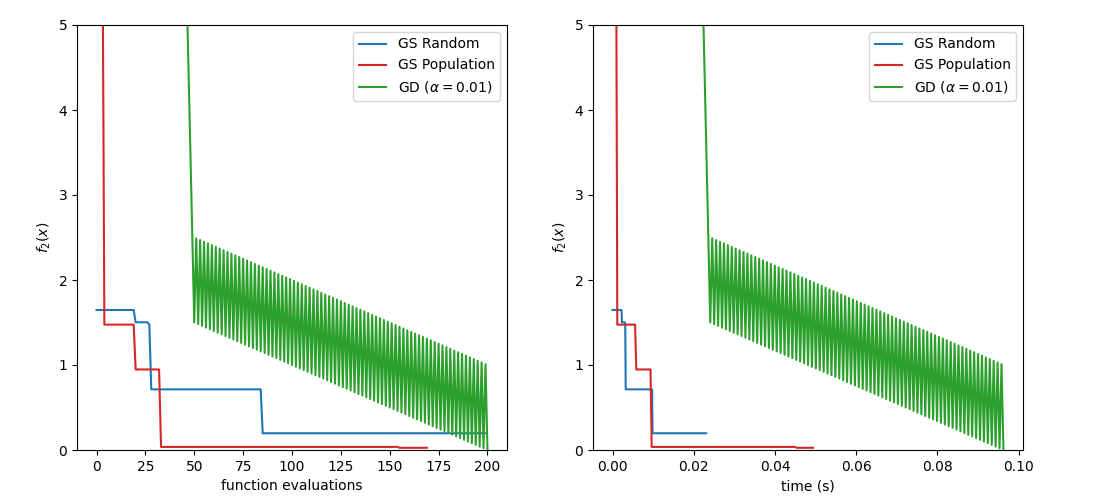
\includegraphics[scale=0.55]{figs/ab/b_ii_2.png}
    \caption{Change in $f_2(x)$ over evaluations and time (GD, GRS and GPS)}
    \label{fig:b_ii_2}
\end{figure}

For $f_2$, the GPS algorithm produces better results than both the GRS and GD algorithms. Like in (a), the GD algorithm oscillates back and forth toward the minimum and never converges while the GRS algorithm fails to find a satisfactory minimum. The GPS algorithm also ran twice as fast as GD making it an even more optimal choice.

\begin{figure}[h]
    \centering
    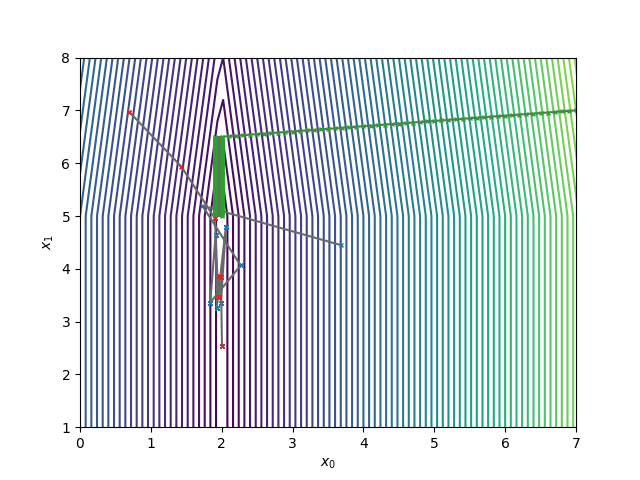
\includegraphics[scale=0.55]{figs/ab/b_ii_2_cont.png}
    \caption{Change in $x$ over evaluations (GD, GRS and GPS)}
    \label{fig:b_ii_2_cont}
\end{figure}

From the contour plot it is clear that the GD algorithm is oscillating back and forth across the minimum ridge while the GPS algorithm finds a minimal point almost immediately.

\section*{Question (c)}

The model compiling and training was moved into its own function which takes, as parameters, the mini-batch size, $\alpha$, $\beta_1$, $\beta_2$ and the number of epochs. It returns the categorical cross-entropy loss of the model. The function can then be passed to the aforementioned GRS and GPS functions to search for optimal hyperparameters. In each case the GPS algorithm was run for 50 iterations while the GPS algorithm was run for 44 iterations ($N=12, M=4, num\_iters=4$).

\noindent \textbf{(i)} A range of mini-batch sizes were searched for in the range $[1, 128]$ while the number of epochs was held constant at 20 and the Adam parameters were kept constant at $\alpha=0.001, \beta_1=0.9, \beta_2=0.999$. 

\begin{figure}[h]
    \centering
    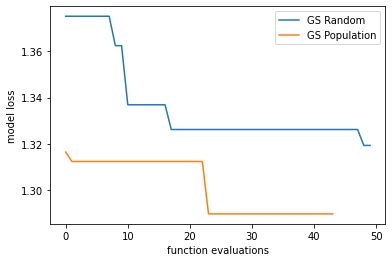
\includegraphics[scale=0.55]{figs/c/c_i.png}
    \caption{Change in model loss over iterations (batch size search)}
    \label{fig:c_i}
\end{figure}

The GPS algorithm performs a good deal better than the GRS algorithm however this does not mean that the GRS algorithm performed poorly. The good performance was most likely due to the parameter search being limited to discrete values as opposed to an effectively infinite continuous range of values. The optimal batch size was found to be 45.

\noindent \textbf{(ii)} A range of Adam parameters were searched for in the ranges $\alpha \in [0.0001, 0.1], \beta_1 \in [0.25, 0.99], \beta_2 \in [0.9, 0.9999]$ while the number of epochs was held constant at 20 and the mini-batch size was set to 45 based on the results of (i).

\begin{figure}[h]
    \centering
    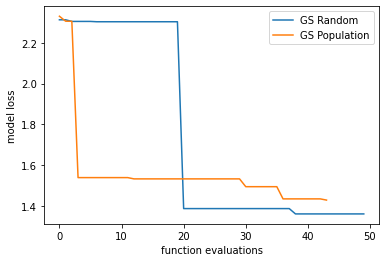
\includegraphics[scale=0.55]{figs/c/c_ii.png}
    \caption{Change in model loss over iterations (Adam parameters search)}
    \label{fig:c_i}
\end{figure}

The GRS algorithm performed slightly better than the GPS algorithm when searching for Adam parameters although neither algorithm produced better results than the default value. The reason for this is most likely due to the parameters being searched for in a uniform way (i.e. random $\alpha$ values closer to 0.0001 are much less likely to appear than values closer to 0.1) this could possibly be generating random values in a logarithmic way.

\noindent \textbf{(iii)} A range of epochs was searched for in the range $[5, 30]$ while the mini-batch size was set to 45 based on the results of (i) and the Adam parameters were kept as the defaults $\alpha=0.001, \beta_1=0.9, \beta_2=0.999$ based on the poor results of (ii).

\begin{figure}[h]
    \centering
    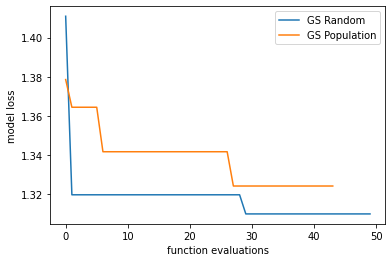
\includegraphics[scale=0.55]{figs/c/c_iii.png}
    \caption{Change in model loss over iterations (epochs search)}
    \label{fig:c_i}
\end{figure}

The GRS algorithm actually performs slightly better than GPS with the former settling on 18 epochs and the latter on 21 epochs. However, neither managed to find the default value of 20 which actually produced a better result.

\newpage

\section*{Appendix A: Code}

\subsection*{Code for (a) and (b)}

\lstset{basicstyle=\footnotesize,xleftmargin=0in}
\lstinputlisting[language=Python]{ab.py}

\subsection*{Code for (c)}

\lstset{basicstyle=\footnotesize,xleftmargin=0in}
\lstinputlisting[language=Python]{c.py}

\end{document}
